\documentclass[a4paper,16pt,oneside,english]{book}
\usepackage[margin=0.5in]{geometry}
\usepackage{hyperref}
\usepackage{fontspec}
\usepackage{etoolbox} % for patchcmd
\usepackage[compact]{titlesec}
\usepackage{minted}
\usepackage{enumitem}
\usepackage{amsmath}
\usepackage{listings}
\usepackage{xcolor}
\usepackage{multicol}
\usepackage{graphicx}
\usepackage{tikz}
\usepackage{xcolor}
\usepackage{etoolbox}
\usepackage{framed}
\usepackage{float}

\hypersetup{
  pdftitle={ITEC50 Web Systems and Technologies Laboratory \#2},
  pdfauthor={Lyra Phasma}
}

\title{ITEC50 Web Systems and Technologies Laboratory \#2}
\author{Lyra Phasma}
\date{February 26, 2026}

\setmainfont[
  Path=assets/static/fonts/,
  UprightFont = *-Regular,
  BoldFont    = *-Bold,
  ItalicFont  = *-RegularItalic,
  BoldItalicFont = *-BoldItalic,
]{Manrope}

\newfontfamily{\LatinModernRoman}{Latin Modern Roman}

\setmonofont[Path=assets/static/fonts/,Scale=0.9]{ComicMono.ttf}

\hyphenpenalty=9999
\exhyphenpenalty=10000
\sloppy
\renewcommand{\arraystretch}{1.5}
\setlength{\emergencystretch}{4em}
\setlength{\parskip}{1em}
\AtBeginEnvironment{tabular}{\fontsize{10}{12}\selectfont}
\titleformat{\chapter}[display]{\normalfont\huge\bfseries}{\chaptertitlename\ \thechapter}{-0.5em}{\Huge}
\titlespacing*{\chapter}
  {0pt}    % left margin
  {-5em}    % space before
  {-0.5em}    % space after
\setlength{\parindent}{0pt}

\renewcommand{\contentsname}{Table of Contents}

\lstdefinestyle{text}{
    basicstyle=\ttfamily\color{black},
    breaklines=true,
}

\definecolor{white}{HTML}{ffffff}
\definecolor{purple}{HTML}{a68cd9}

\makeatletter

% PATCH: CHAPTER
\patchcmd{\chapter}{\if@openright\cleardoublepage\else\clearpage\fi}{}{}{}
\let\old@chapter\chapter
\renewcommand{\chapter}{%
  \ifdim\pagetotal=0pt % remove margin if it's at top of page
    \vspace*{-2.5em}
  \fi
  \@ifstar
    {\old@chapter*}
    {\old@chapter}%
}
\titleformat{\chapter} % or [block]
  {\normalfont\LARGE\bfseries}
  {\thechapter}{0.625em}{}
\titlespacing*{\chapter}
  {0pt}    % left margin
  {0em}    % space before
  {-0.5em}    % space after

\makeatother

\usemintedstyle{tango}
\newcommand{\inputmintedstyled}[2]{%
  \inputminted[
    fontsize=\small,
    fontfamily=tt,
    bgcolor=white,
    rulecolor=\color{purple},
    linenos,
    numbersep=10pt,
    frame=single,
    framesep=2mm,
    breaklines,
    tabsize=4,
    breakafter=-/,
    breakbefore=\,\\
  ]{#1}{#2}%
}

\newcommand{\inputmintedstyledtwocolumns}[2]{%
  \begin{multicols}{2}
  \inputminted[
    fontsize=\small,
    fontfamily=tt,
    bgcolor=white,
    rulecolor=\color{purple},
    linenos,
    numbersep=0pt,
    frame=single,
    framesep=2mm,
    breaklines,
    tabsize=4,
    breakafter=-/,
    breakbefore=\,\\
  ]{#1}{#2}
  \end{multicols}%
}

\newcommand{\quotefont}{\rmfamily}

\newcommand*\quotesize{80} % if quote size changes, need a way to make shifts relative
% Make commands for the quotes
\newcommand*{\openquote}
   {\tikz[remember picture,overlay,xshift=-2.5ex,yshift=-4.5ex]
   \node (OQ) {\quotefont\fontsize{\quotesize}{\quotesize}\selectfont``};\kern0pt}

\newcommand*{\closequote}[1]
  {\tikz[remember picture,overlay,xshift=2.5ex,yshift={#1}]
   \node (CQ) {\quotefont\fontsize{\quotesize}{\quotesize}\selectfont''};}

% select a colour for the shading
\colorlet{shadecolor}{gray!10}

\newcommand*\shadedauthorformat{\emph} % define format for the author argument

% Now a command to allow left, right and centre alignment of the author
\newcommand*\authoralign[1]{%
  \if#1l
    \def\authorfill{}\def\quotefill{\hfill}
  \else
    \if#1r
      \def\authorfill{\hfill}\def\quotefill{}
    \else
      \if#1c
        \gdef\authorfill{\hfill}\def\quotefill{\hfill}
      \else\typeout{Invalid option}
      \fi
    \fi
  \fi}
% wrap everything in its own environment which takes one argument (author) and one optional argument
% specifying the alignment [l, r or c]
%
\newenvironment{shadequote}[2][l]%
{
\vspace{1em}
\authoralign{#1}
 \ifblank{#2}
   {\def\shadequoteauthor{}\def\yshift{-1ex}\def\quotefill{\hfill}}
   {\def\shadequoteauthor{\par\authorfill\shadedauthorformat{#2}}\def\yshift{-2ex}}
 \begin{snugshade}\vspace{0.25em}\begin{quote}\openquote}
{\shadequoteauthor\quotefill\closequote{\yshift}\end{quote}\end{snugshade}%
}

\begin{document}

{
  \centering
  {\huge ITEC50 Web Systems and Technologies\par}
  {\Huge Laboratory \#2\par}
}

\noindent
\begin{minipage}{0.5\textwidth}
\raggedright
Lyra Phasma
\end{minipage}
\begin{minipage}{0.5\textwidth}
\raggedleft
ITEC50\\
February 26, 2026
\end{minipage}


\tableofcontents

\listoffigures

\listoftables

\chapter{Declaration of Academic Integrity}

I affirm that all work in this document that is not explicitly attributed to others is entirely my own, including code, explanations, and problem solutions. Any external assistance (tutorials, references, templates, or AI guidance) is clearly indicated in the Article "Attributions." All sources, where known, are cited to maintain academic integrity.

Artificial intelligence assistance was used solely for formatting guidance in {\LatinModernRoman \LaTeX}. The work presented herein are entirely my own work.

\chapter{Introduction}

This document may appear lengthy at first glance. However, the majority of its pages consist of screenshots included to demonstrate the responsiveness and consistency of the website across different layouts and scenarios.

As the live website will be publicly accessible under my newly registered domain \url{https://lyra-on.top}, it is associated with my online nickname and pen name, "Lyra Phasma." This identity allows me to maintain privacy and personal safety, particularly given the challenges I face as a member of a sexual minority, while also enabling a highly visible portfolio for academic evaluation, professional opportunities, and personal projects. Accordingly, any personal identifiers in this document (such as legal name or student ID) are intentionally omitted in publicly shared versions, including the first page—which contains the official laboratory description and grading rubric—while complete identifying information is provided through official submission channels.

At the time of submission, the domain may not yet be publicly accessible due to hosting arrangements. Once deployment is finalized, I will promptly notify the instructor so that the live version may be reviewed if desired. The complete project source code is also maintained in a GitHub repository (https://github.com/whinee/ITEC50-Lab-2) for transparency and version control.

This document is organized to clearly present both the visual output and underlying implementation of the project. Each webpage section first includes screenshots demonstrating layout and responsiveness across different screen resolutions, followed immediately by the corresponding HTML source code. This structure allows the reader to directly associate the rendered result with the markup that produced it.

The Cascading Stylesheet (CSS) files are presented in a separate chapter, as they are shared across multiple pages and function as the styling foundation of the website.

The final chapters include proper attributions for external resources used in the project, as well as the complete {\LatinModernRoman \LaTeX} source code of this document for full transparency regarding its preparation and formatting.

\textit{Note: Some sections of this report may appear extensive or detailed beyond strict laboratory requirements. This reflects both a thorough demonstration of implementation and, admittedly, my personal enthusiasm for the technologies involved.}

\newpage

\chapter{Pages}

\section{\texttt{404.html}}

\subsection{Screenshots}

\begin{figure}[H]
  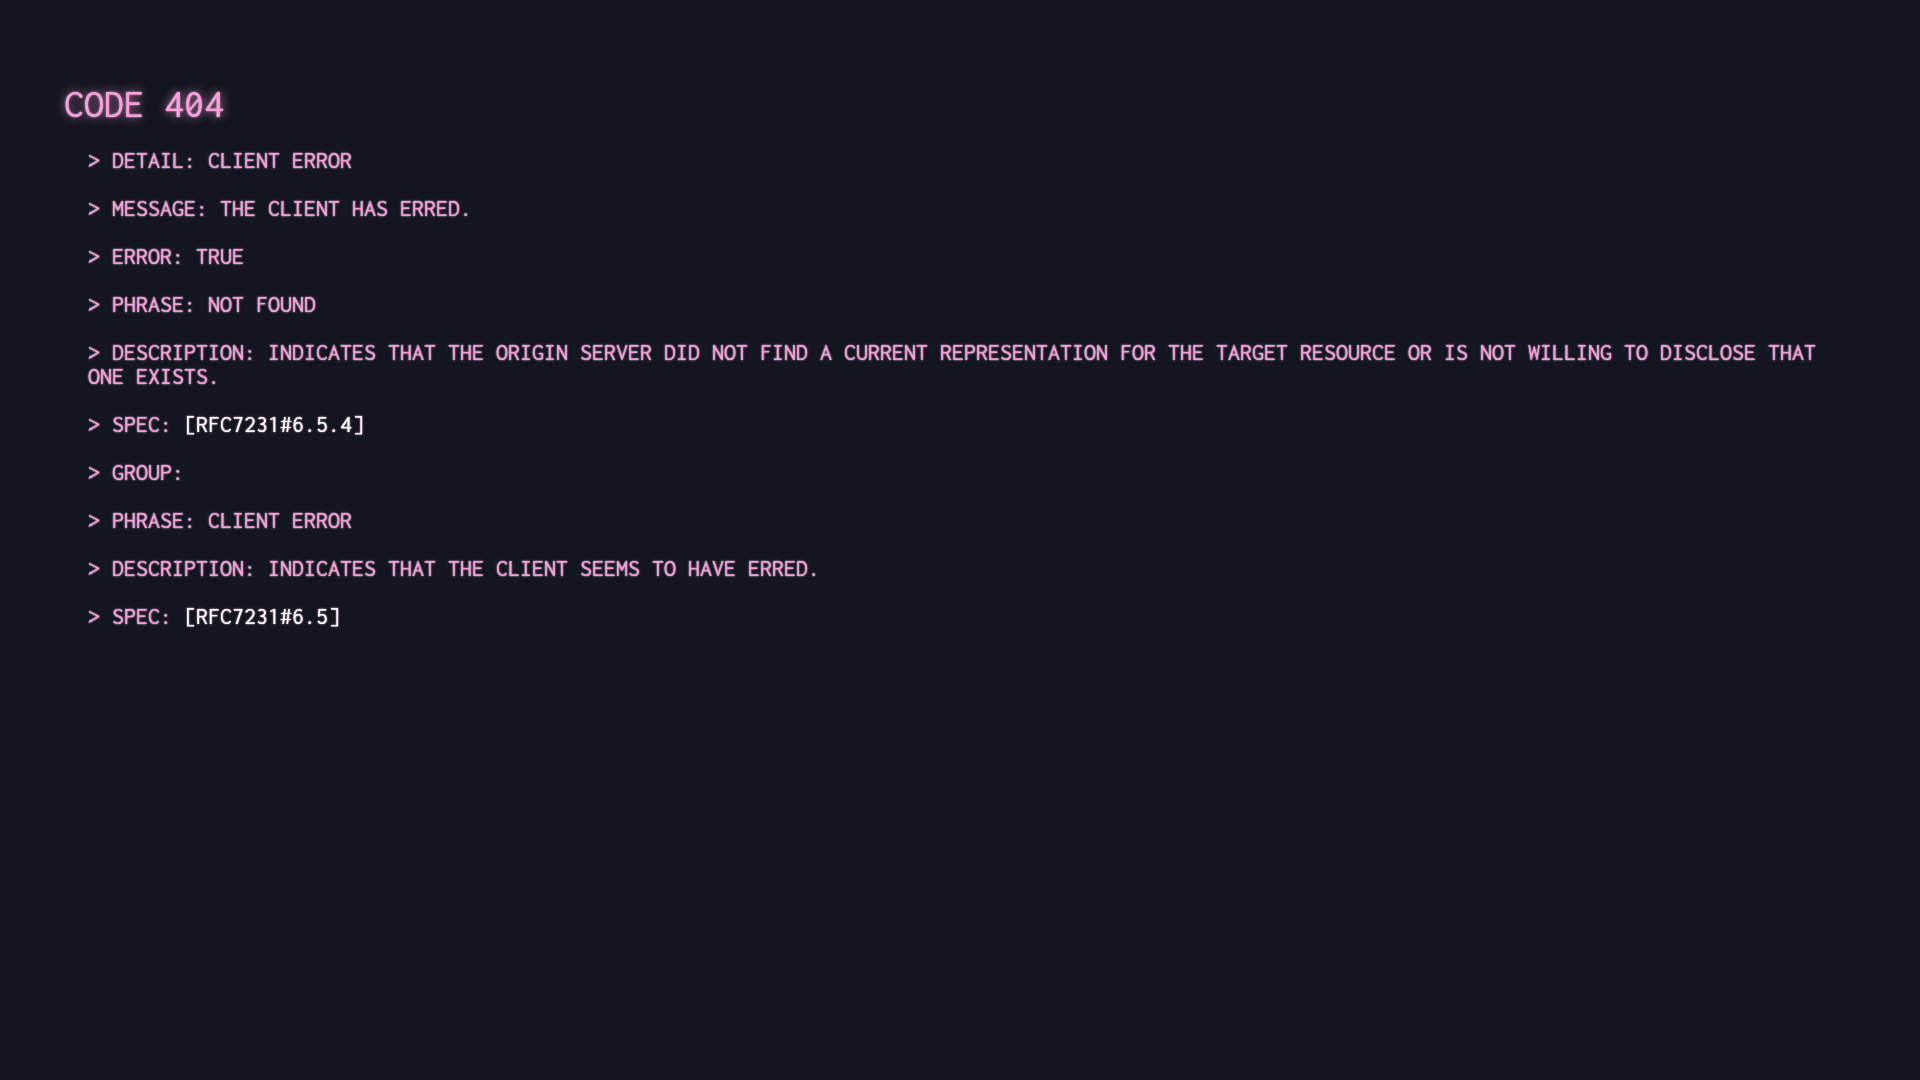
\includegraphics[width=\linewidth]{assets/static/images/screenshots/404.html.png}
  \caption{404.html 1920x1080 px}
  \label{fig:404-html}
\end{figure}

\begin{figure}[H]
  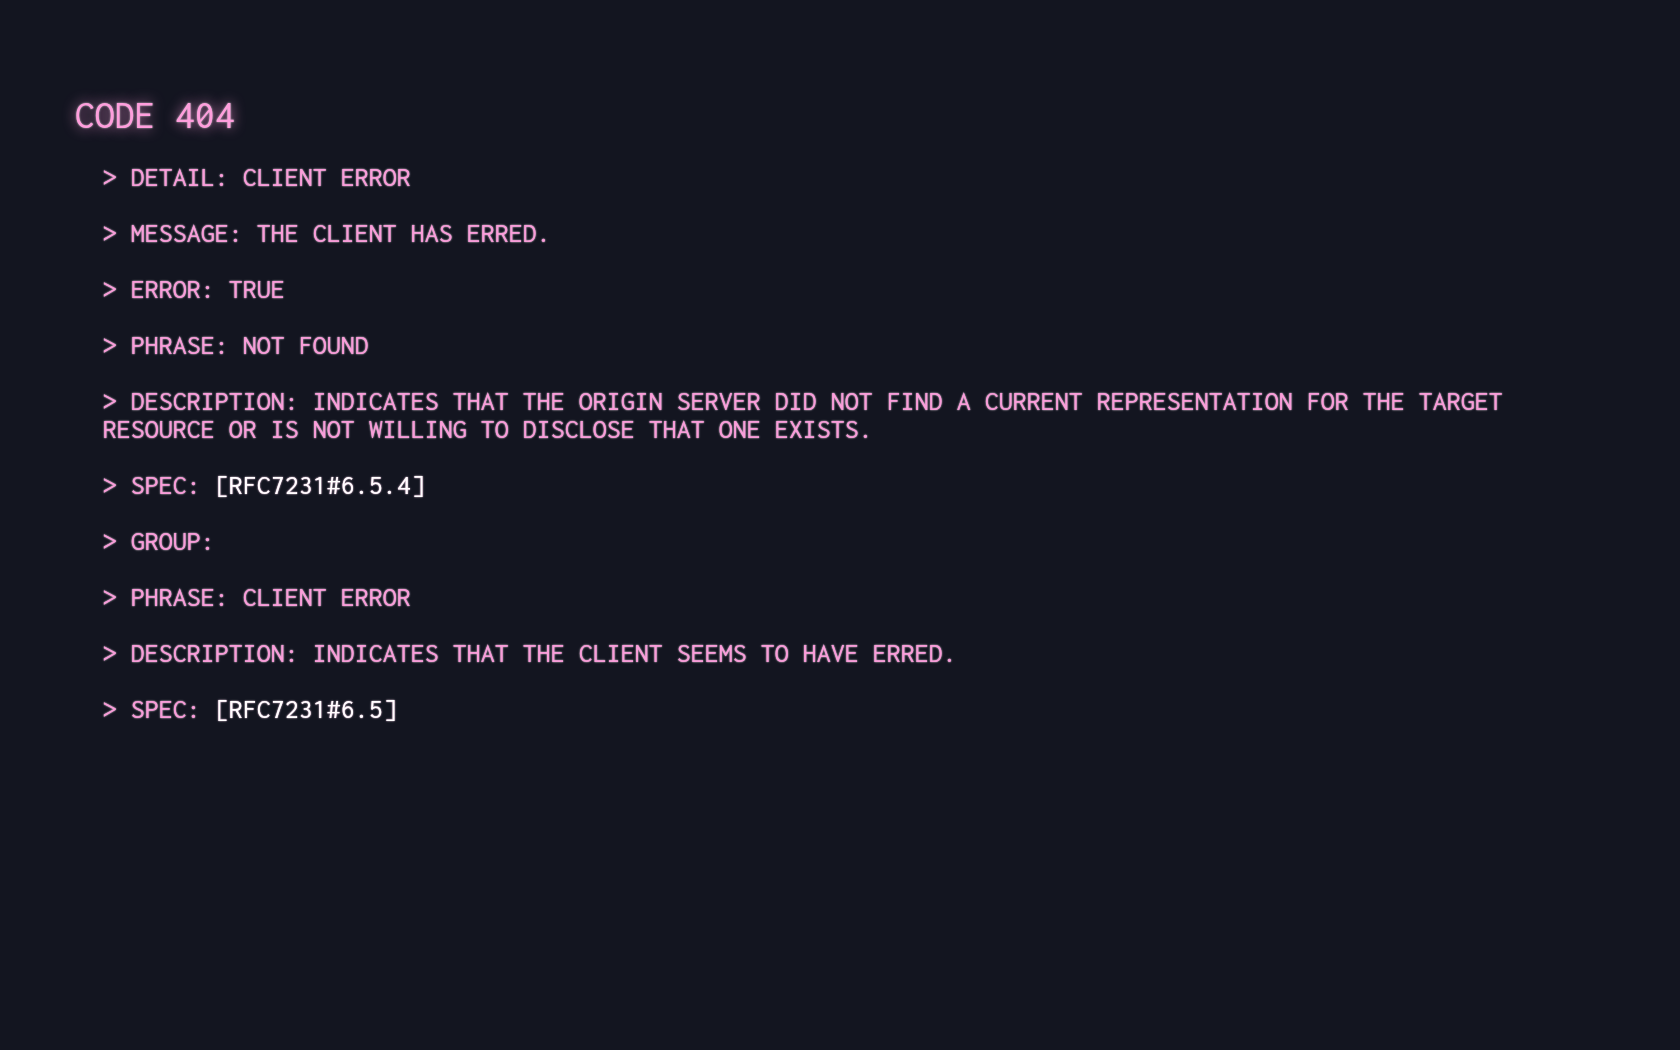
\includegraphics[width=\linewidth]{assets/static/images/screenshots/404.html-1680x1050.png}
  \caption{404.html 1680x1050}
  \label{fig:404.html-1680x1050}
\end{figure}

\begin{figure}[H]
  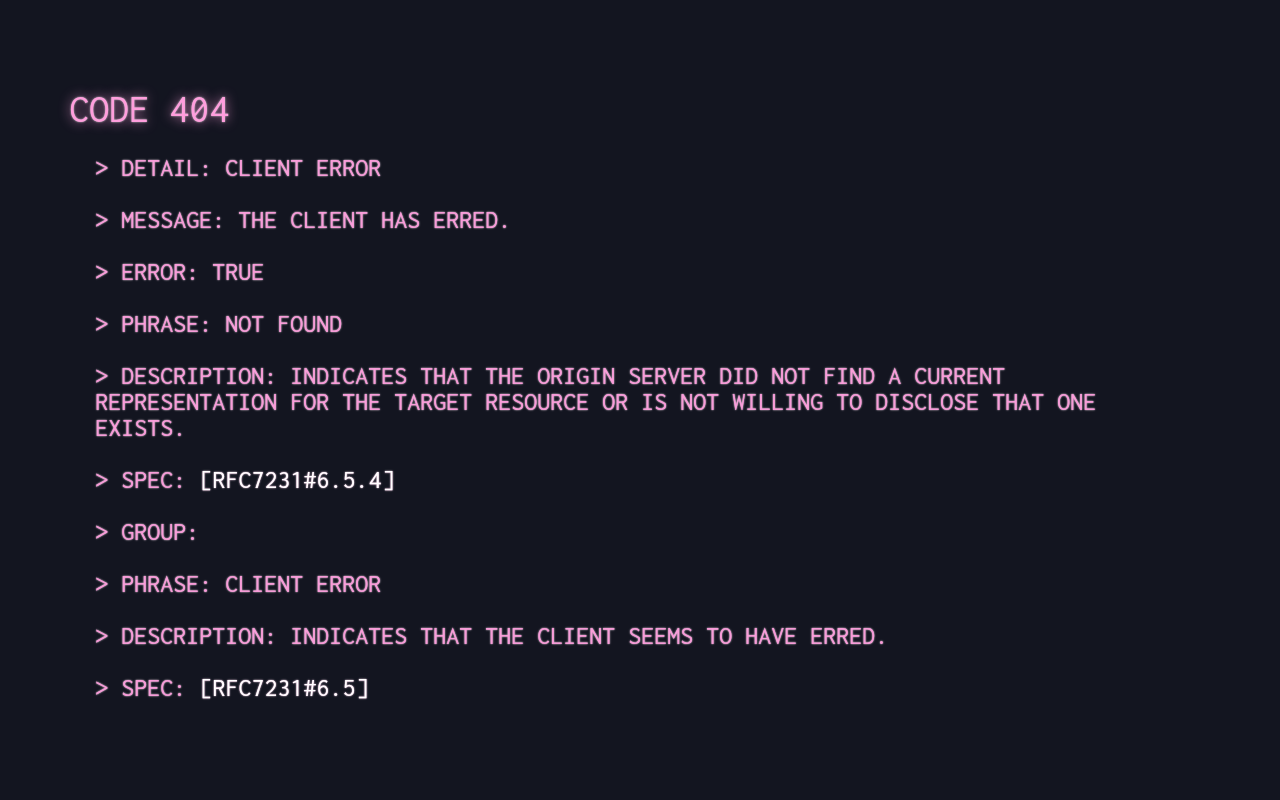
\includegraphics[width=\linewidth]{assets/static/images/screenshots/404.html-1280x800.png}
  \caption{404.html 1280x800 px}
  \label{fig:404.html-1280x800}
\end{figure}

\begin{figure}[H]
  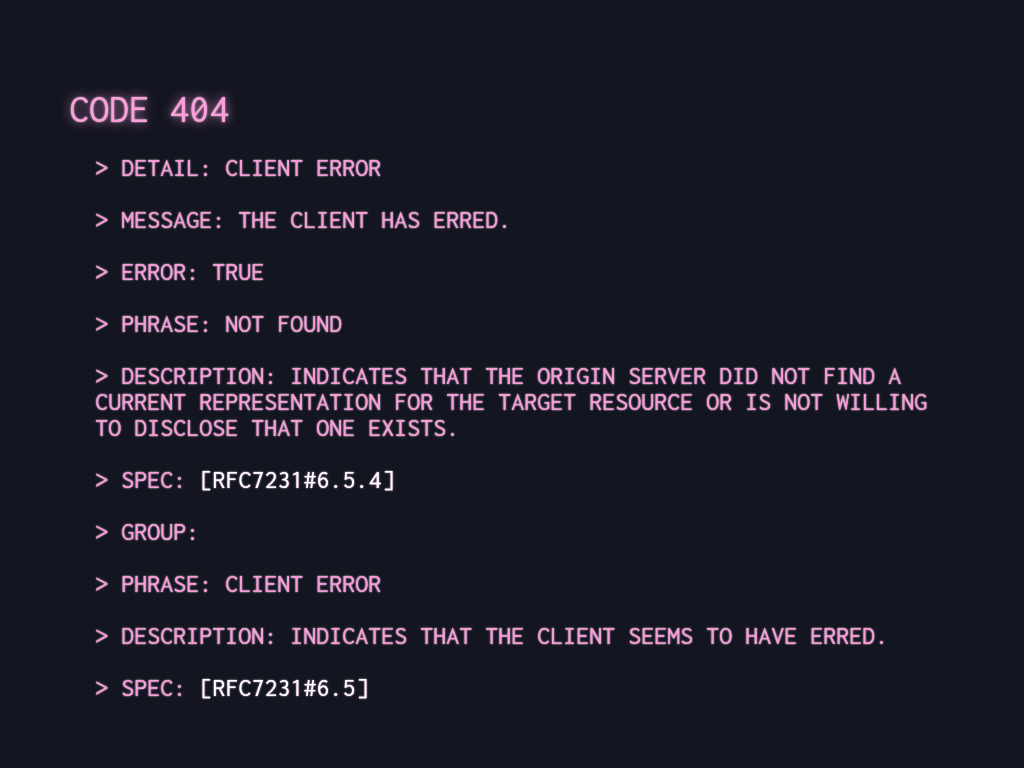
\includegraphics[width=\linewidth]{assets/static/images/screenshots/404.html-1024x768.png}
  \caption{404.html 1024x768 px}
  \label{fig:404.html-1024x768}
\end{figure}

\begin{figure}[H]
  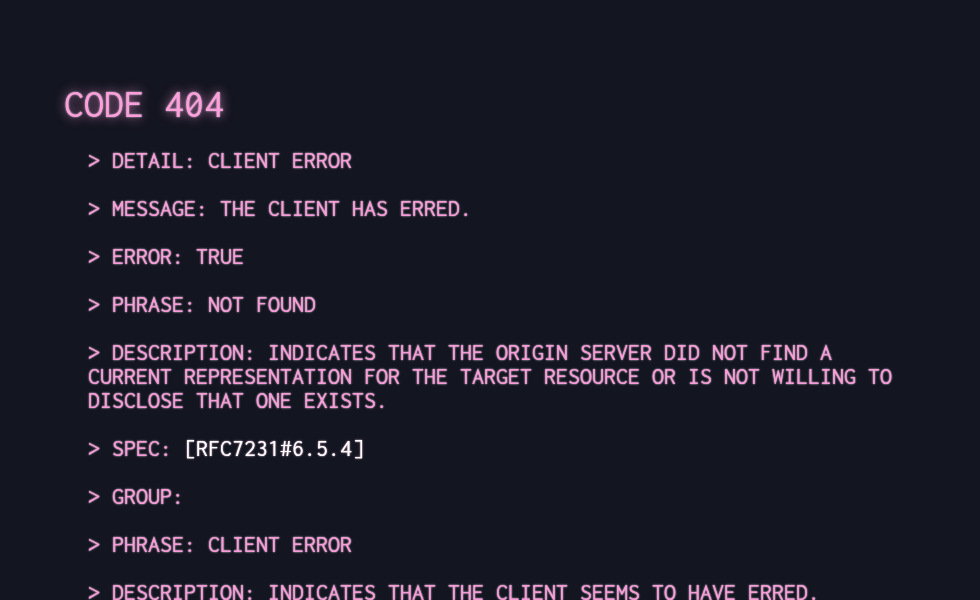
\includegraphics[width=\linewidth]{assets/static/images/screenshots/404.html-980x600.png}
  \caption{404.html 980x600 px}
  \label{fig:404.html-980x600}
\end{figure}

\begin{figure}[H]
  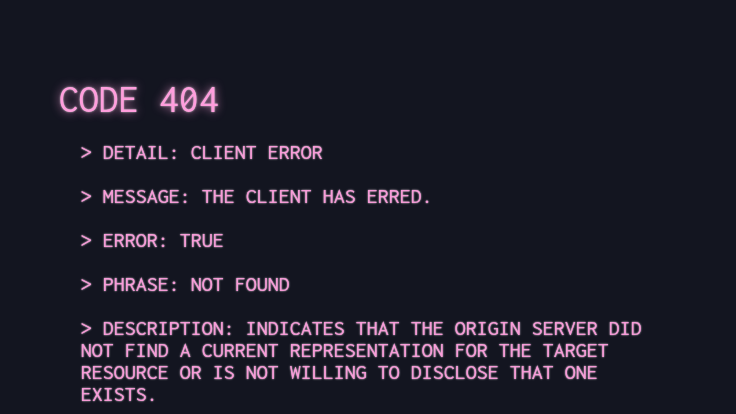
\includegraphics[width=\linewidth]{assets/static/images/screenshots/404.html-736x414.png}
  \caption{404.html 736x414 px}
  \label{fig:404.html-736x414}
\end{figure}

\begin{figure}[H]
  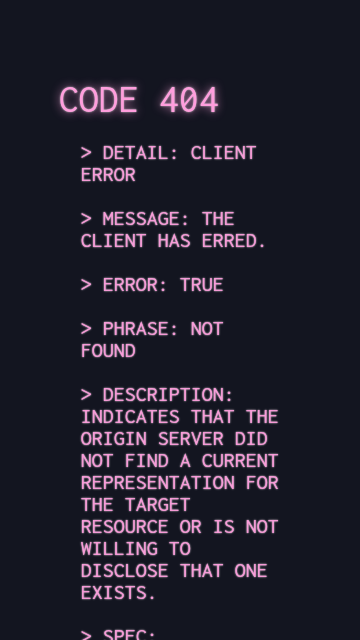
\includegraphics[height=0.85\paperheight]{assets/static/images/screenshots/404.html-360x640.png}
  \caption{404.html 360x640 px}
  \label{fig:404.html-360x640}
\end{figure}

\subsection{HTML Source Code}

\inputmintedstyled{html}{404.html}

\newpage

\section{\texttt{index.html}}

\subsection{Screenshots}

\begin{figure}[H]
  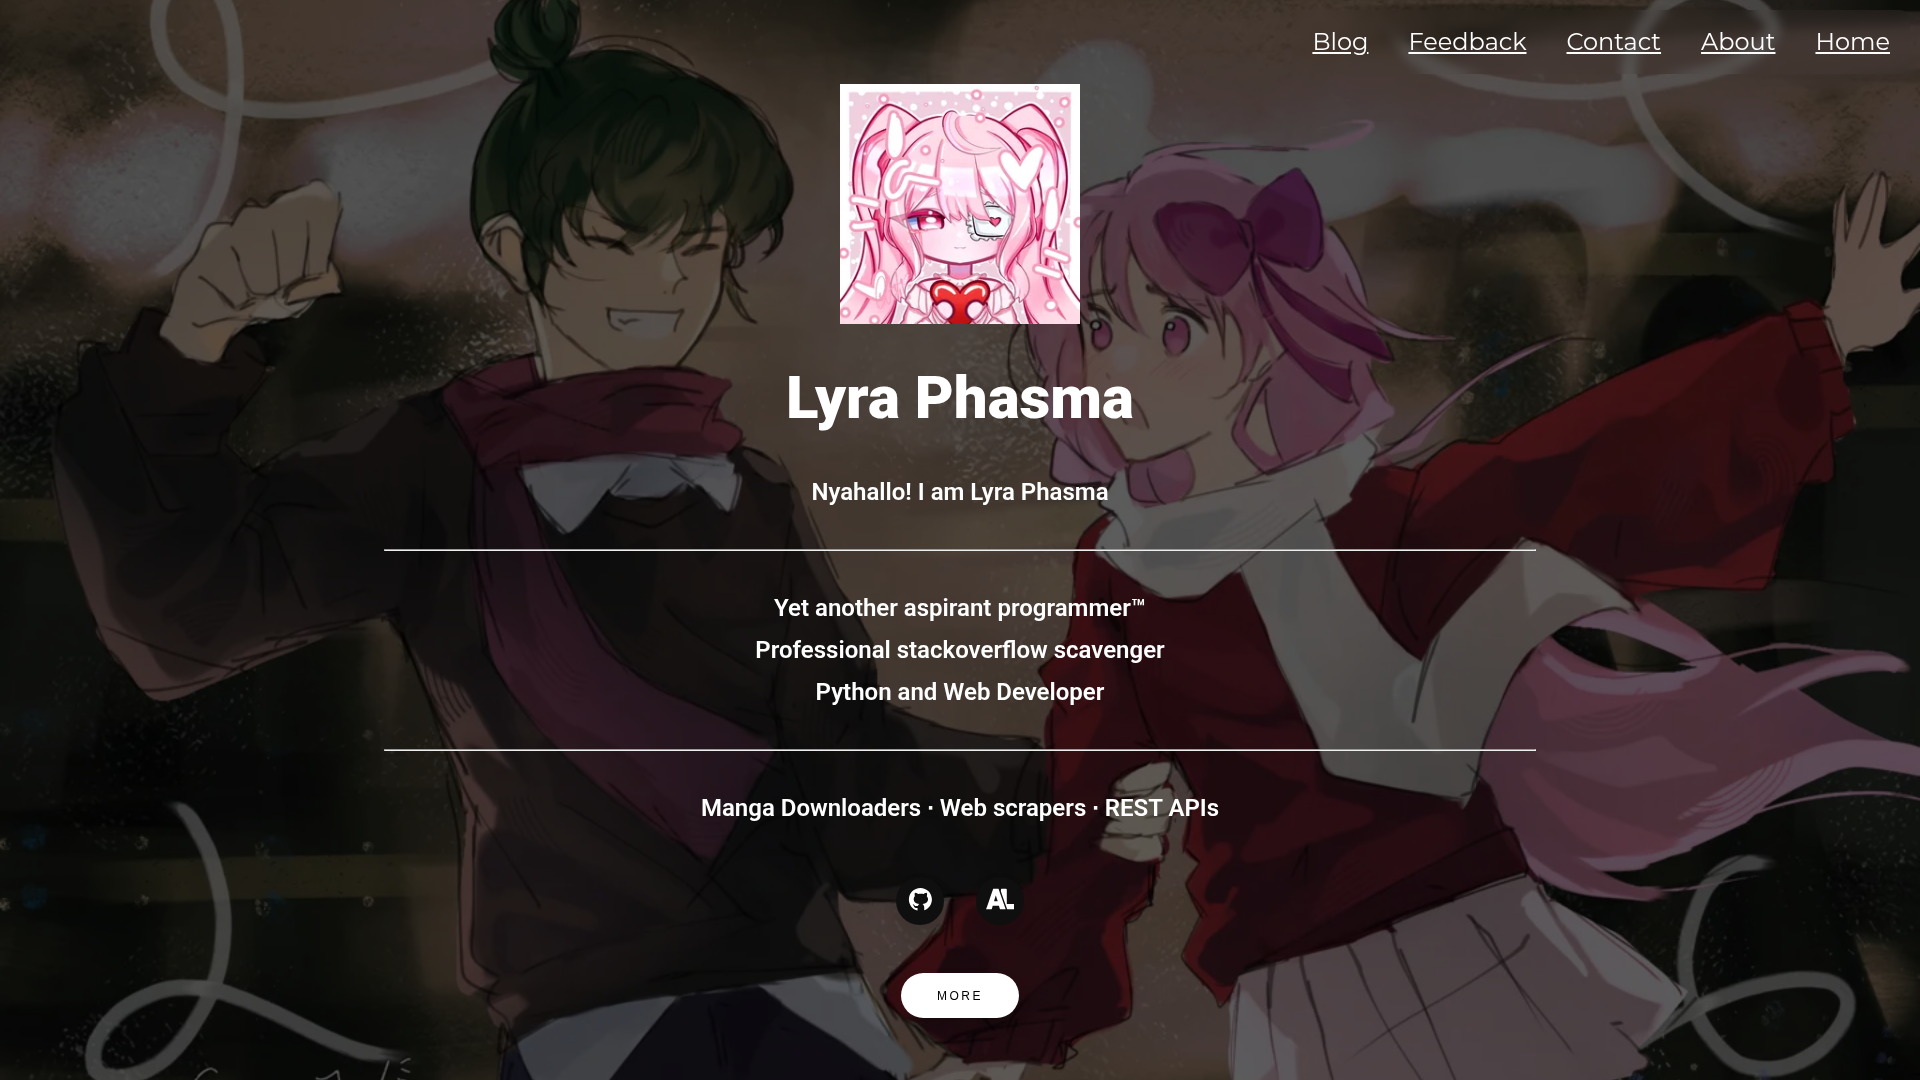
\includegraphics[width=\linewidth]{assets/static/images/screenshots/index.html.png}
  \caption{index.html 1920x1080 px}
  \label{fig:index-html}
\end{figure}

\begin{figure}[H]
  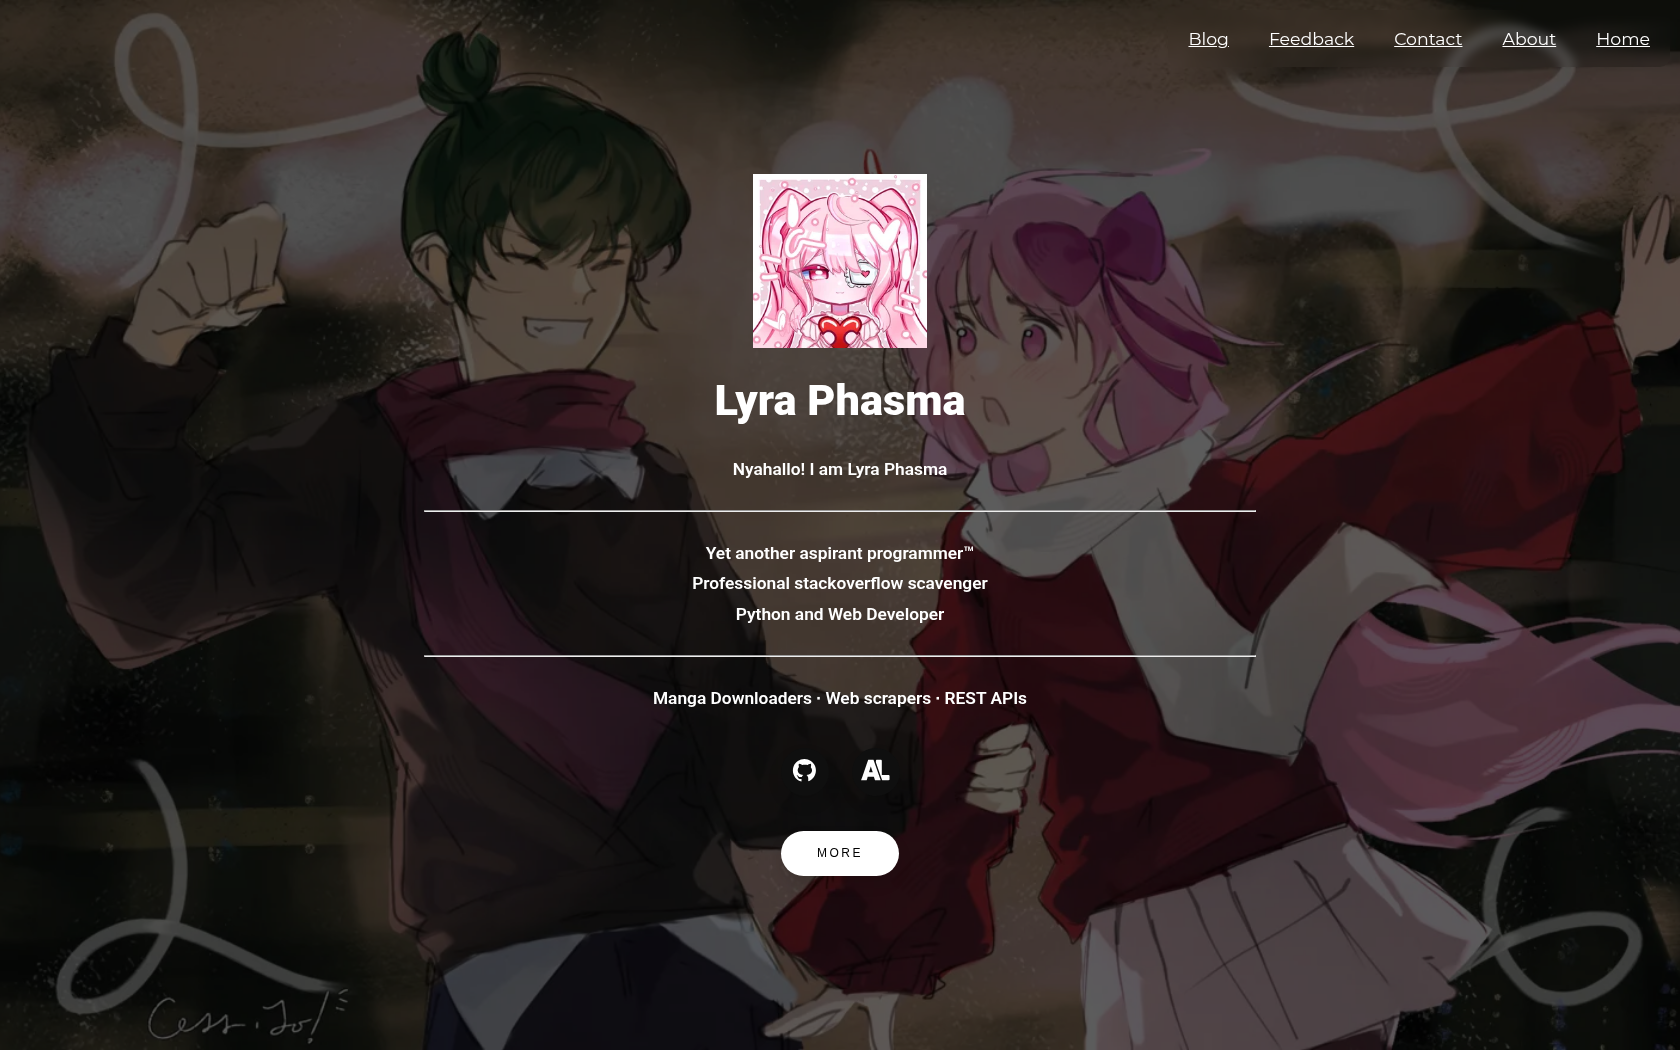
\includegraphics[width=\linewidth]{assets/static/images/screenshots/index.html-1680x1050.png}
  \caption{index.html 1680x1050 px}
  \label{fig:index.html-1680x1050}
\end{figure}

\begin{figure}[H]
  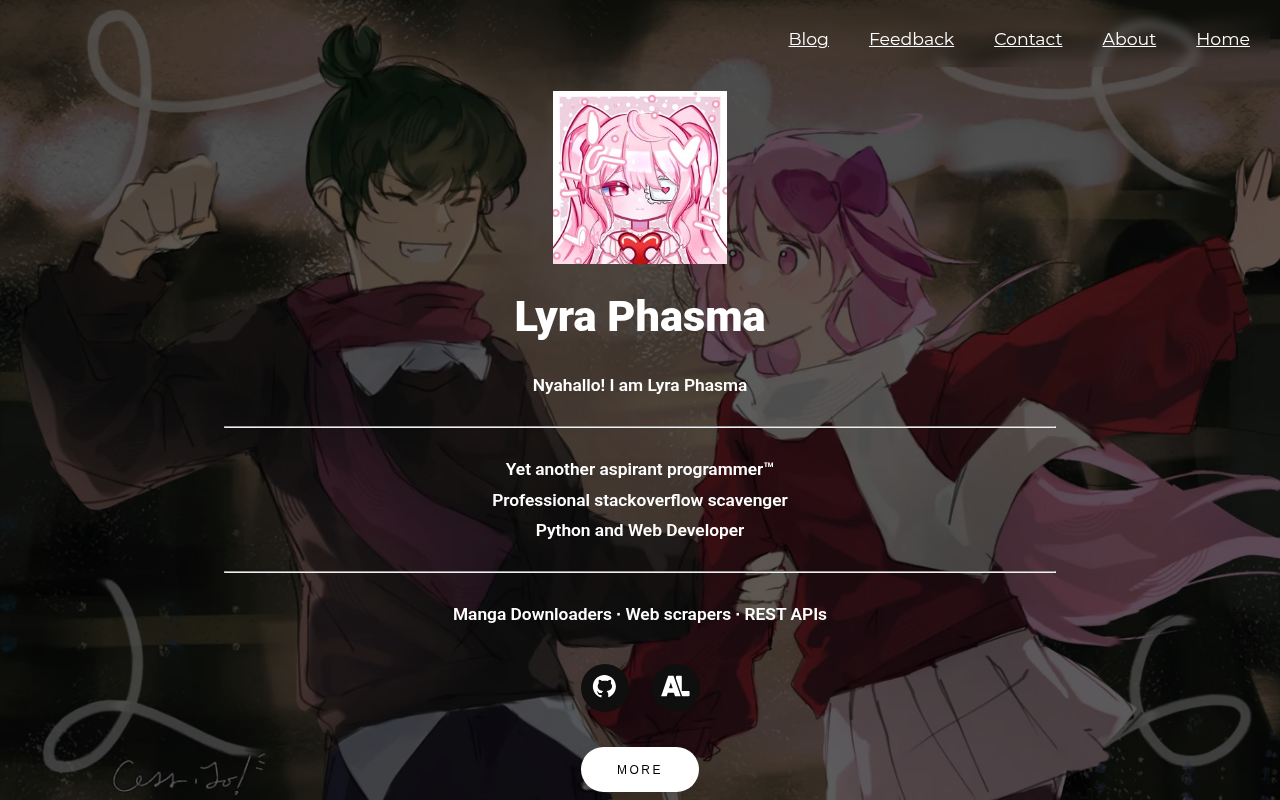
\includegraphics[width=\linewidth]{assets/static/images/screenshots/index.html-1280x800.png}
  \caption{index.html 1280x800 px}
  \label{fig:index.html-1280x800}
\end{figure}

\begin{figure}[H]
  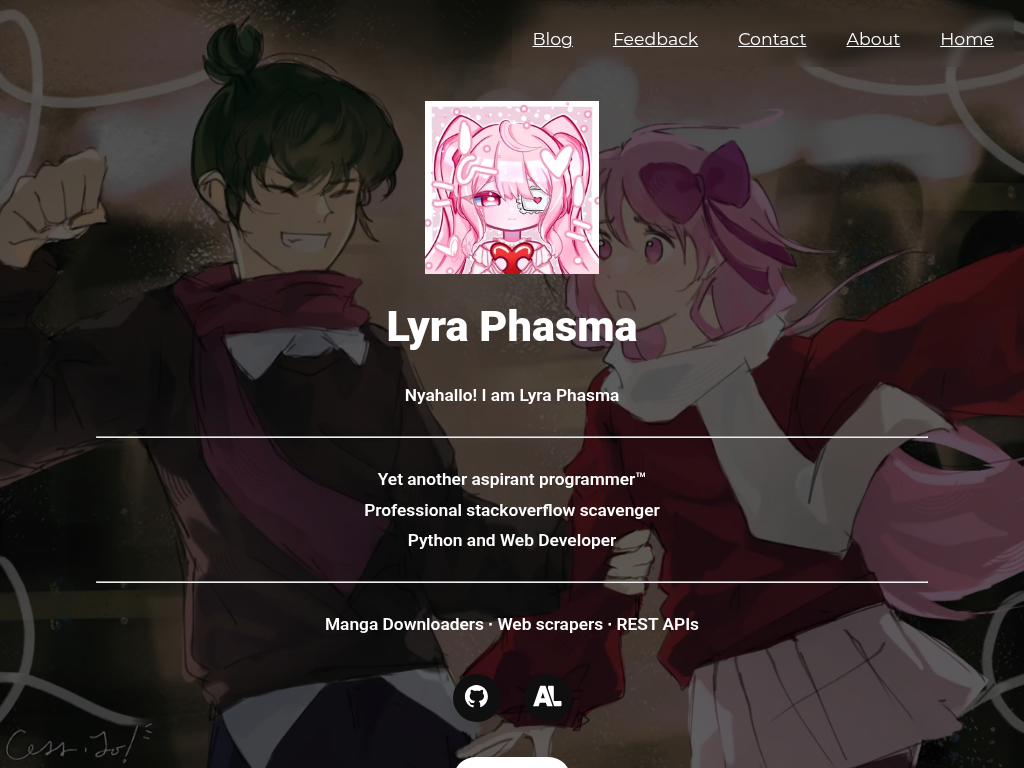
\includegraphics[width=\linewidth]{assets/static/images/screenshots/index.html-1024x768.png}
  \caption{index.html 1024x768 px}
  \label{fig:index.html-1024x768}
\end{figure}

\begin{figure}[H]
  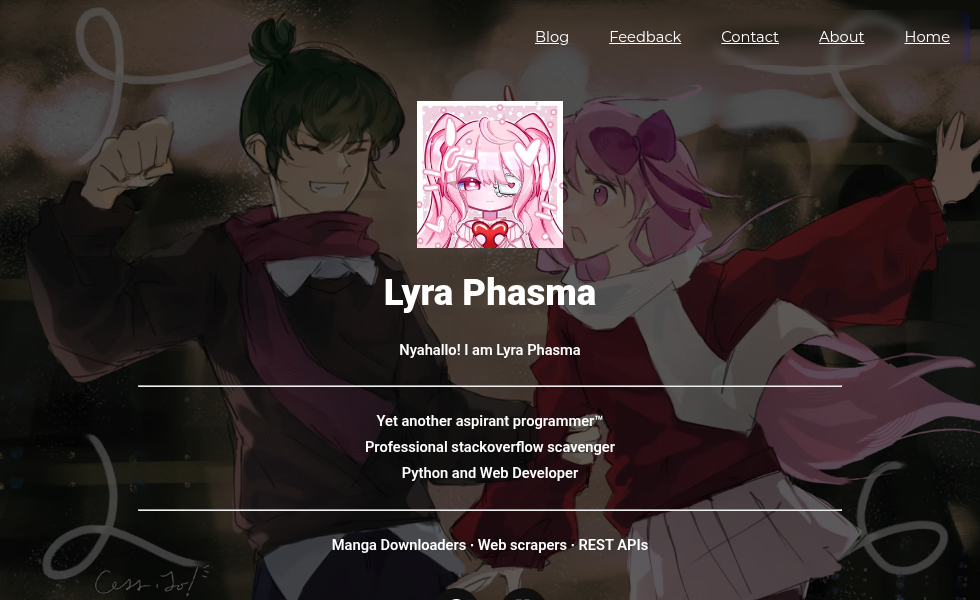
\includegraphics[width=\linewidth]{assets/static/images/screenshots/index.html-980x600.png}
  \caption{index.html 980x600 px}
  \label{fig:index.html-980x600}
\end{figure}

\begin{figure}[H]
  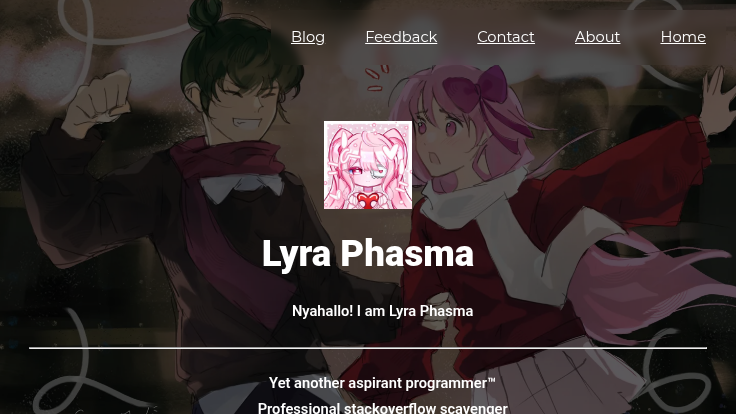
\includegraphics[width=\linewidth]{assets/static/images/screenshots/index.html-736x414.png}
  \caption{index.html 736x414 px}
  \label{fig:index.html-736x414}
\end{figure}

\begin{figure}[H]
  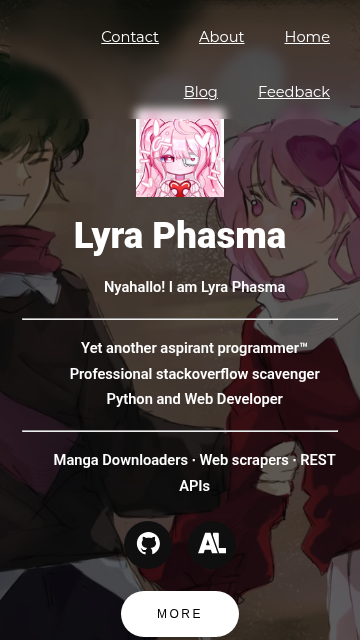
\includegraphics[height=0.85\paperheight]{assets/static/images/screenshots/index.html-360x640.png}
  \caption{index.html 360x640 px}
  \label{fig:index.html-360x640}
\end{figure}

\subsection{HTML Source Code}

\inputmintedstyled{html}{index.html}

\newpage

\chapter{Lighthouse Reports}

Lighthouse is a tool developed by Google that audits web pages across several important dimensions, including performance, accessibility, adherence to best practices, and search engine optimization (SEO). It provides quantitative metrics such as First Contentful Paint (FCP), Largest Contentful Paint (LCP), Time to Interactive (TTI), Total Blocking Time (TBT), and Cumulative Layout Shift (CLS), which together give a clear picture of how quickly and reliably a webpage loads, becomes usable, and remains visually stable. Accessibility scores highlight whether users with disabilities can effectively navigate and interact with the site, while best practices and SEO checks ensure modern web standards and discoverability are maintained.

\begin{multicols}{2}

% Automatically generated Lighthouse report for all pages

\section{\texttt{blog/00011.html}}

    \begin{table}[H]
    \centering
    \caption{Lighthouse Scores for blog/00011.html}
    \begin{tabular}{|l|c|}
    \hline
    Category & Score \\ \hline
    Performance & 61 \\ \hline
    Accessibility & 86 \\ \hline
    Best Practices & 92 \\ \hline
    SEO & 100 \\ \hline
    \end{tabular}
    \end{table}

    \begin{table}[H]
    \centering
    \caption{Lighthouse Metrics for blog/00011.html}
    \begin{tabular}{|l|c|}
    \hline
    Metric & Value \\ \hline
    FCP & 3.5 s \\ \hline
    LCP & 4.1 s \\ \hline
    SpeedIndex & 3.5 s \\ \hline
    TTI & 4.1 s \\ \hline
    TBT & 0 ms \\ \hline
    CLS & 0 \\ \hline
    \end{tabular}
    \end{table}
    \section{\texttt{blog/index.html}}

    \begin{table}[H]
    \centering
    \caption{Lighthouse Scores for blog/index.html}
    \begin{tabular}{|l|c|}
    \hline
    Category & Score \\ \hline
    Performance & 61 \\ \hline
    Accessibility & 87 \\ \hline
    Best Practices & 92 \\ \hline
    SEO & 100 \\ \hline
    \end{tabular}
    \end{table}

    \begin{table}[H]
    \centering
    \caption{Lighthouse Metrics for blog/index.html}
    \begin{tabular}{|l|c|}
    \hline
    Metric & Value \\ \hline
    FCP & 3.5 s \\ \hline
    LCP & 4.1 s \\ \hline
    SpeedIndex & 3.5 s \\ \hline
    TTI & 4.1 s \\ \hline
    TBT & 0 ms \\ \hline
    CLS & 0 \\ \hline
    \end{tabular}
    \end{table}
    \section{\texttt{404.html}}

    \begin{table}[H]
    \centering
    \caption{Lighthouse Scores for 404.html}
    \begin{tabular}{|l|c|}
    \hline
    Category & Score \\ \hline
    Performance & 64 \\ \hline
    Accessibility & 67 \\ \hline
    Best Practices & 96 \\ \hline
    SEO & 100 \\ \hline
    \end{tabular}
    \end{table}

    \begin{table}[H]
    \centering
    \caption{Lighthouse Metrics for 404.html}
    \begin{tabular}{|l|c|}
    \hline
    Metric & Value \\ \hline
    FCP & 3.0 s \\ \hline
    LCP & 3.6 s \\ \hline
    SpeedIndex & 3.0 s \\ \hline
    TTI & 3.6 s \\ \hline
    TBT & 0 ms \\ \hline
    CLS & 0 \\ \hline
    \end{tabular}
    \end{table}
    \section{\texttt{about.html}}

    \begin{table}[H]
    \centering
    \caption{Lighthouse Scores for about.html}
    \begin{tabular}{|l|c|}
    \hline
    Category & Score \\ \hline
    Performance & 59 \\ \hline
    Accessibility & 87 \\ \hline
    Best Practices & 92 \\ \hline
    SEO & 100 \\ \hline
    \end{tabular}
    \end{table}

    \begin{table}[H]
    \centering
    \caption{Lighthouse Metrics for about.html}
    \begin{tabular}{|l|c|}
    \hline
    Metric & Value \\ \hline
    FCP & 3.8 s \\ \hline
    LCP & 4.7 s \\ \hline
    SpeedIndex & 3.8 s \\ \hline
    TTI & 4.7 s \\ \hline
    TBT & 0 ms \\ \hline
    CLS & 0 \\ \hline
    \end{tabular}
    \end{table}
    \section{\texttt{contact.html}}

    \begin{table}[H]
    \centering
    \caption{Lighthouse Scores for contact.html}
    \begin{tabular}{|l|c|}
    \hline
    Category & Score \\ \hline
    Performance & 59 \\ \hline
    Accessibility & 88 \\ \hline
    Best Practices & 96 \\ \hline
    SEO & 100 \\ \hline
    \end{tabular}
    \end{table}

    \begin{table}[H]
    \centering
    \caption{Lighthouse Metrics for contact.html}
    \begin{tabular}{|l|c|}
    \hline
    Metric & Value \\ \hline
    FCP & 3.8 s \\ \hline
    LCP & 4.7 s \\ \hline
    SpeedIndex & 3.8 s \\ \hline
    TTI & 4.7 s \\ \hline
    TBT & 0 ms \\ \hline
    CLS & 0 \\ \hline
    \end{tabular}
    \end{table}
    \section{\texttt{feedback.html}}

    \begin{table}[H]
    \centering
    \caption{Lighthouse Scores for feedback.html}
    \begin{tabular}{|l|c|}
    \hline
    Category & Score \\ \hline
    Performance & 59 \\ \hline
    Accessibility & 88 \\ \hline
    Best Practices & 96 \\ \hline
    SEO & 100 \\ \hline
    \end{tabular}
    \end{table}

    \begin{table}[H]
    \centering
    \caption{Lighthouse Metrics for feedback.html}
    \begin{tabular}{|l|c|}
    \hline
    Metric & Value \\ \hline
    FCP & 3.8 s \\ \hline
    LCP & 4.7 s \\ \hline
    SpeedIndex & 3.8 s \\ \hline
    TTI & 4.7 s \\ \hline
    TBT & 0 ms \\ \hline
    CLS & 0 \\ \hline
    \end{tabular}
    \end{table}
    \section{\texttt{index.html}}

    \begin{table}[H]
    \centering
    \caption{Lighthouse Scores for index.html}
    \begin{tabular}{|l|c|}
    \hline
    Category & Score \\ \hline
    Performance & 59 \\ \hline
    Accessibility & 72 \\ \hline
    Best Practices & 96 \\ \hline
    SEO & 92 \\ \hline
    \end{tabular}
    \end{table}

    \begin{table}[H]
    \centering
    \caption{Lighthouse Metrics for index.html}
    \begin{tabular}{|l|c|}
    \hline
    Metric & Value \\ \hline
    FCP & 3.8 s \\ \hline
    LCP & 4.8 s \\ \hline
    SpeedIndex & 3.8 s \\ \hline
    TTI & 4.8 s \\ \hline
    TBT & 0 ms \\ \hline
    CLS & 0.001 \\ \hline
    \end{tabular}
    \end{table}
    

\end{multicols}

\clearpage

\chapter{Cascading Stylesheets (CSS) Files}

\section{\texttt{assets/static/stylesheets/base.css}}

Notice that there are no \texttt{!important} imperative in \texttt{assets/static/stylesheets/base.css}? That is intentional. It serves as the basis of styling for all the homepages, and thus, if a specific page has a different requirement from that of the base stylesheet, then it can be easily overriden by a \texttt{!important} imperative.

\inputmintedstyledtwocolumns{css}{assets/static/stylesheets/base.css}
\newpage

\section{\texttt{assets/static/stylesheets/code.css}}
\inputmintedstyledtwocolumns{css}{assets/static/stylesheets/code.css}
\newpage

\section{\texttt{assets/static/stylesheets/home.css}}
\inputmintedstyledtwocolumns{css}{assets/static/stylesheets/home.css}
\newpage

\section{\texttt{assets/static/stylesheets/responsive-base.css}}
\inputmintedstyledtwocolumns{css}{assets/static/stylesheets/responsive-base.css}
\newpage

\chapter{Attributions}

\section{Artwork}

All artworks remain the intellectual property of their respective creators and are included in this academic submission with permission.

The artworks used in this project are as follows:

\subsection{Artwork by Cess\_.2}

Cess\_.2. (December 29, 2025). \textit{Untitled artwork} [Digital illustration].

\textbf{Official pages:}
\begin{itemize}
    \item https://www.facebook.com/Cesstwo44
    \item https://www.instagram.com/zesy.to
\end{itemize}

The file is located relative to the project’s root directory at \\
\texttt{assets/static/images/Lyra-and-Dreanne-Night-Market-Cess\_.2.png}.

Usage permissions granted by mutual agreement with the artist:

\begin{shadequote}{}
You may download and possess this work for personal, non-commercial, non-public use.\\
No redistribution, modification, or derivative works allowed.\\
All rights are retained by the artist.
\end{shadequote}

\subsection{Artwork by Asterope}

Asterope. (n.d.). \textit{Untitled artwork} [Digital illustration].

\textbf{Official page:}
\begin{itemize}
    \item https://www.facebook.com/Nyxstarry2
\end{itemize}

The file is located relative to the project’s root directory at  
\texttt{assets/static/images/PFP-Asterope.png}.

This artwork was created specifically for the author and is used with the artist’s permission.  
All copyright remains with the original creator.  
No redistribution or derivative use is permitted without the artist’s consent.

\section{Fonts}

The fonts used in this document are the following:

Sharanda M. (2018). \textit{Manrope} [Font]. Licensed under the SIL Open Font License, Version 1.1. Retrieved June 5, 2025, from https://fonts.google.com/specimen/Manrope.

Voos M. (2020). \textit{Manrope Italic} [Font]. Licensed under the SIL Open Font License, Version 1.1. Retrieved June 14, 2025, from https://github.com/malte-v/manrope-italic.

Pangsakulyanont T. (2018). \textit{Comic Mono} [Font]. Licensed under the MIT License. Retrieved June 5, 2025, from https://github.com/dtinth/comic-mono-font.

\appendix

\newpage

\chapter{Source Code for this Document}

\inputmintedstyledtwocolumns{latex}{main.tex}

\end{document}